
\documentclass{aa}  

%
\usepackage{graphicx}
\usepackage[table]{xcolor}
%%%%%%%%%%%%%%%%%%%%%%%%%%%%%%%%%%%%%%%%
\usepackage{txfonts}
\usepackage{bm}
\usepackage{multirow, makecell}
\usepackage{booktabs}
\usepackage{fontawesome}
\newcommand{\github}{\href{https://github.com/dlanzieri/WL_Implicit-Inference}{\faGithub}} %For Denise: Remember to label the final version of the Github repo with the notebook
%%%%%%%%%%%%%%%%%%%%%%%%%%%%%%%%%%%%%%%%

\usepackage[colorlinks=true,citecolor=blue,linkcolor=blue,urlcolor=blue]{hyperref}
\begin{document} 

\title{Optimal Neural Summarisation for Full-Field Implicit Inference by Density Estimation }

\newcommand{\justine}[1]{{\color{cyan}JZ: #1}}
\newcommand{\denise}[1]{{\color{red}DL: #1}}
\newcommand{\FL}[1]{{\color{magenta}FL: #1}}
\newcommand{\LM}[1]{{\color{olive}LM: #1}}

\author{Denise Lanzieri \inst{1}
\and
Justine Zeghal \inst{2}
\and
T. Lucas Makinen \inst{3}
\and
Alexandre Boucaud \inst{2}
\and
Fran\c{c}ois Lanusse \inst{4}
\and
Jean-Luc Starck \inst{4}
}
\institute{Université Paris Cité, Université Paris-Saclay, CEA, CNRS, AIM, F-91191, Gif-sur-Yvette, France
\and
Université Paris Cité, CNRS, Astroparticule et Cosmologie, F-75013 Paris, France
\and Imperial Centre for Inference and Cosmology (ICIC) $\&$ Astrophysics Group, Imperial College London, Blackett Laboratory, Prince Consort Road, London SW7 2AZ, United Kingdom
\and
Université Paris-Saclay, Université Paris Cité, CEA, CNRS, AIM, 91191, Gif-sur-Yvette, France
}
\titlerunning{}
\date{Received xxx; accepted xxx}


 
  \abstract
  % context heading (optional)
  % {} leave it empty if necessary  
   {In many cosmological applications, the likelihood function is either unknown or intractable, limiting the use of traditional inference methods. Likelihood-Free Inference (LFI) approaches offer a promising solution by using forward-simulated synthetic data to approximate the posterior (or likelihood) distribution instead of evaluating an explicit likelihood function. However, these methods suffer from the curse of dimensionality, necessitating the development of compression schemes to reduce high-dimensional data into lower-dimensional summary statistics.

%    \justine{\textbf{I think the 2 main ideas for this part are: }

%     - classical way to overcome this issue: we compress the data into 2pt statistics  and use gaussian likelihood → pb: we miss a lot of information}
%     \denise{That's true. But adding it in the abstract would make the "Context" subsection (this division is mandatory for A$\&$A) too long. This is properly described in the introduction}
    
%     \justine{ - considering the previous pb: thanks to Implicit Inference methods we can consider any kind of summary stat (because we can learn the exact posterior p(theta | summary stat)), so to have the best contours (meaning that we exatrct all gaussian as well as non-gaussian signal) we only have to focus on how we compress our data.}
%     \denise{That's also true. But we don't use any summary statistics (except the power spectrum because it's easy), and I think that one of the points of the paper is to extract the information from the pixels, without using any summaries. So I personally would not talk about summary statistics }


%      \justine{\textbf{Note:}
    
%     - for me LFI = Implicit Inference, I think we should use only one
%    }
%    \denise{True again. But the definition "Likelihood-Free Inference" is more used in the community. Implicit Inference is something that we introduce in the motivation and introduction. I don't know exactly how much people are familiar with this concept. }
%     \justine{ - 'Likelihood-Free Inference (LFI) approaches offer a promising solution by using forward-simulated synthetic data instead of an explicit likelihood function.' → Implicit inference approaches offer a promising solution to approximate posterior distribution by using simulations from an implicit likelihood (a simulator) instead of evaluating explicit likelihood function ..?

%     - I'm probably wrong but not sure about the last sentence.
% }
   }   
  % aims heading (mandatory)
    {We aim to derive the optimal neural-compression strategy for full field Likelihood free inference by density estimation. Moreover, by using the optimal compression strategy, we demonstrate that the posterior distribution is comparable to those derived from a Bayesian forward modeling approach.}  
  % methods heading (mandatory)
    { We present a comparative analysis of different loss functions employed during the training of the neural network. We  evaluate their performance by measuring their impact on the constraints on the $\Lambda$CDM parameters expected from LSST-Y10.
    For both forward-modeling the convergence field and generating observed mock data, we use the \href{https://github.com/DifferentiableUniverseInitiative/sbi_lens}{\url{SbiLens}} package. 
    \texttt{SbiLens} is a jax-based differentiable physical model specifically designed for Likelihood Free Inference and Bayesian inference algorithms that require access to likelihood derivatives.
    
    % \justine{\textbf{I think the main ideas for this part are: }

    % - first we describe sbi\_lens : Provides a differentiable log normal mass map simulator specifically designed for for weak lensing inference. Then you can describe a bit the simulations like tomographic bins etc I guess
    
    
    % - We construct our ground truth
    
    
    % - We use implicit inference techniques to go from the compressed stat to the posteriors}
    }
  % results heading (mandatory)
   {Our experiments validate the effectiveness of LFI methods,  as we demonstrate comparable posterior distributions between LFI and Bayesian forward modeling approaches.
   % \justine{field-based Bayesian Hierarchical Model analysis}. 
   Additionally, our results provide insights into the design of data compression procedures to derive low-dimensional summary statistics while minimizing information loss. All codes associated with this paper can be found at this link \github.}
  % conclusions heading (optional), leave it empty if necessary 
   {}
   \keywords{methods: statistical – gravitational lensing: weak – cosmology: large-scale structure of Universe
               }


   \maketitle

%-------------------------------------------------------------------
%------------------------------------------------------------------
%------------------------------------------------------------------
%------------------------------------------------------------------
\section{Introduction}
Weak gravitational lensing by the large-scale structure is caused by the presence of foreground matter bending the light emitted by background galaxies. Being sensitive to the large-scale structure of the universe, it is one of the most promising tools for investigating the nature of dark energy, the origin of the accelerating expansion of the universe and estimating cosmological parameters. Future cosmological surveys, such as the Legacy Survey of Space and Time (LSST) of the Vera C. Rubin Observatory \citep{ivezic2019lsst}, the Nancy Grace Roman Space Telescope \citep{spergel2015wide}, and  the Euclid Mission \citep{laureijs2011euclid}, will rely on weak gravitational lensing as one of the principal physical probes to address unresolved questions in current cosmology.
 As these surveys become deeper, they will be able to access more non-Gaussian features of the matter fields. This makes the standard weak lensing analyses, which rely on two-point statistics such as the 2-point shear correlation or the angular power spectrum, sub-optimal. These analyses are unable to fully capture the non-Gaussian information imprinted in the lensing signal and can only access Gaussian information.


To overcome this limitation, several higher-order statistics have been introduced. These include weak lensing peak counts \citep{liu2015cosmology,  liu2015cosmological, lin2015new, kacprzak2016cosmology, peel2017cosmological, shan2018kids, martinet2018kids, ajani2020constraining, harnois2021cosmic, zurcher2022dark}, wavelet and scattering transform \citep{ajani2021starlet, cheng2021weak}, the one point PDF \citep{liu2019constraining, uhlemann2020fisher, boyle2021nuw}, Minkowski functionals \citep{kratochvil2012probing, petri2013cosmology}, moments of mass maps \citep{gatti2021dark},  and 3 point statistics \citep{takada2004cosmological, semboloni2011weak, rizzato2019tomographic, halder2021integrated}. 
Although these methods have proven to improve cosmological constraints, they rely on summary statistics, for which an analytical description is often lacking. These methods frequently assume a Gaussian likelihood and require accurate computation of the covariance matrix, which can be challenging.



One way to overcome the use of summary statistics and bypass the associated issues, such as the use of simplified and unjustified likelihood assumptions, is through the use of map-based approaches.
Within this category, a further distinction can be made between methods that integrate observations into a forward model allowing the exact reconstruction of the likelihood, and those designed to directly reconstruct the likelihood from synthetic data as part of the inference pipeline.
The former scenario, often referred to as Bayesian forward-modeling,  has gained popularity in the literature in the last decades \citep{schneider2015hierarchical, alsing2016hierarchical, alsing2017cosmological, bohm2017bayesian, porqueres2021bayesian, porqueres2022lifting, porqueres2023field}. Despite the differences among these works in terms of the physical models they assume or the specific quantities they aim to sample, they all demonstrate that conducting a field-level analysis results in more precise and accurate constraints compared to the two-point function analysis.
Despite the immense potential of these approaches, there is a noteworthy limitation: they frequently result in high-dimensional problems, necessitating the use of sophisticated statistical sampling techniques. \\
An alternative framework for inference is provided by Likelihood-Free Inference (LFI) approaches, which are sometimes referred to as Likelihood implicit or Simulation-Based Inference (SBI). Increasingly employed in astrophysics and cosmology \citep{lin2015new, alsing2018generalized, jeffrey2021likelihood, gerardi2021unbiased, tam2022likelihood}, the potential of LFI methods lies in the fact that they primarily rely on our ability to forward-simulate synthetic data, without the need for an explicit likelihood function. As a result, these methods are free from assumptions and approximations. Furthermore, incorporating systematic effects and complex physical processes into forward simulations is more straightforward compared to including them when constructing the likelihood function.
Given the potential of LFI methods, it is crucial to identify possible sources of bias and the associated challenges. For instance, it is widely recognized that even the most advanced LFI methods can be affected by the curse of dimensionality. This necessitates compression procedures that reduce the high-dimensional data set into a small number of summary statistics.
A significant question is how to design data compression procedures, aiming to derive low-dimensional summary statistics while minimizing information loss. Moreover, it is imperative to establish well-defined procedures to validate the results.



In this paper, we present a comparison of the performance of various neural network-based compression schemes within the Likelihood-Free Inference (LFI) framework. These methods differ in terms of the loss functions used to train the neural network, but they share the same inference strategy based on neural density estimation. To address the need for result validation in the LFI context, we employ a Bayesian forward modeling approach that enables inference on the joint posterior of the cosmological parameters and the convergence field. The forward model is based on \href{https://github.com/DifferentiableUniverseInitiative/sbi_lens}{\url{SbiLens}}, a Python package designed for weak lensing inference with differentiable simulator implemented in Jax. \texttt{SbiLens} allows the sampling of convergence maps in a tomographic setting, accounting for the cross-correlation between different redshift bins.



The paper is structured as follows: in \autoref{Sec:Motivation}, we illustrate the motivation behind this work. In \autoref{Sec:the SBILens framework}, we introduce the \texttt{SbiLens} framework and describe the simulated data used in this work. In \autoref{Sec:experiment}, we detail the inference strategy and the three different approaches we used: the power spectrum, the map-based inference based on the Bayesian forward-modeling, and the map-based inference based on the LFI. In the same section, we also provide a detailed overview of different neural compression strategies. In \autoref{Sec:results}, we discuss the results and validate the LFI approaches. Finally, we conclude in \autoref{Sec:conclusion}. 
%------------------------------------------------------------------
%------------------------------------------------------------------
%------------------------------------------------------------------
%------------------------------------------------------------------
\section{Motivation}\label{Sec:Motivation}
%--------------------------------------------------------------------
With the increased statistical power of stage IV surveys, our cosmological analysis should not rely on the measurement of sub-optimal summary statistics, that may not fully capture the non-Gaussian information present in the lensing field at the scales accessible to future surveys. In this paper we introduce a forward model that directly extracts information from the raw pixel data, rather than relying on the analytical evaluation of summary statistics. By doing so, we aim to preserve all available information and facilitate the incorporation of systematic effects and the combination of multiple cosmological probes through joint simulations.
In this context, the simulator of the observables serves as our physical model, where each component is tractable. These models, often refereed to as \textit{probabilistic program}, can be described as follows. They take as input a vector parameter $\bm{\theta}$, which describes the underlying deterministic model. Then, they sample internal states, dubbed \textit{latent variables}, from the distribution $\bm{z}_i \sim p_i(\bm{z}_i|\bm \theta, \bm{z}_{<i})$, that can be directly or indirectly related to a physically meaningful state of the system. Finally, they generate the output $\bm x$ from the distribution $\ p(\bm d|\bm \theta)$, where $\bm{d}$ represents the observations. 


The ultimate goal of Bayesian inference in cosmology is to compute the posterior distribution:
\begin{equation}\label{Eq:posterior}
     p(\bm{\theta}|\bm{x})= 
     \frac{p(\bm{x}|\bm{\theta})p(\bm{\theta})}
     {\int d\bm{\theta'}p(\bm{x}|\bm{\theta}')p(\bm{\theta}')},
\end{equation}
however, a problems arises because the marginal likelihood $p(\bm{x}|\bm{\theta})$ is typically intractable:
\begin{equation}
    p(\bm{x}|\bm{\theta})=\int p(\bm{x},\bm{z}|\bm{\theta}) d\bm{z}=\int p(\bm{x}|\bm{z},\bm{\theta})p(\bm{z}|\bm{\theta}) d\bm{z}.
\end{equation}
as it corresponds to an integral over all possible trajectories throughout the latent space.
To overcome this limitation while still capturing the full information content of the data, two different approaches have been proposed in the literature. Although these approaches are often referred to by different names, in this work, we will make the following distinction:
%--------------------------------------------------------------------
\paragraph{\textbf{Explicit inference}} referring to all Likelihood-based inference approaches.  
This approach involves treating the simulator as a probabilistic model and performing inference over the joint posterior:
\begin{equation}
        p(\bm{\theta},\bm{z}|\bm{x})\propto  p(\bm{x},\bm{z}|\bm{\theta}) p(\bm{z}|\bm{\theta}).
\end{equation}
In the context of the forward model and full field analysis, fall in this category the Bayesian Hierarchical Models (BHMs).
A Bayesian forward approach involves using a given physical model to predict observations and then comparing these predictions with observations to infer the parameters of the model.
However, performing a global analysis on complex and large datasets, such as a lensing dataset, is not feasible. Therefore, the idea of dividing the global analysis into several subgroups, analyzing them in multiple steps, and using the output of each of those as input for the next one. From here, the \textit{hierarchical} nature of this methodology.
%--------------------------------------------------------------------
\paragraph{\textbf{Implicit inference}} referring to all the approaches not relying on an analytical model to describe the signal, but rather on learning the likelihood from simulations. This second class of approaches involves treating the simulator as a black box with only the ability to sample from the joint distribution:
\begin{equation}
    (\bm{x}, \bm{\theta})\sim p(\bm{x}, \bm{\theta}).
\end{equation}
Within this class of methods, we can differentiate between more traditional methods such as Approximate Bayesian Computation (ABC) and Density Estimation Likelihood-Free Inference (DELFI) methods. ABC employs rejection-criteria based approaches to approximate the likelihood by comparing simulations with data. 
In this work, our focus will be on DELFI methods, which approach the inference task as a density estimation problem. \\
We can divide Likelihood-Free Inference approaches into two separate steps:
\begin{enumerate}
    \item  Automatically learning an optimal low-dimensional summary statistic.
    \item Using Neural Density Estimation in low dimensions to infer the target distributions.
\end{enumerate}
In the first step, we introduce a parametric function $f_{\varphi}$ such that:
     \begin{equation}
         \bm{t}=F_{\varphi}(\bm{\theta}),
     \end{equation}
which aims to reduce the dimensionality of the data while preserving information. Typically, the compressed statistics $\bm{t}$ is assumed to have the same dimension of $\bm{\theta}$. \\
In the second step, Neural Density Estimation can target either building an estimate $p_{\phi}$ of the likelihood function $p(\bm{x}|\bm{\theta})$ (referred to as the Neural Likelihood Estimation (NLE) task), or targeting the posterior distribution $p(\bm{\theta}|\bm{x})$, (known as Neural Posterior Estimation (NPE) task). 

It is important to note that not all neural compression techniques are equivalent. Many papers that apply neural techniques for extracting summary statistics have used sub-optimal compression techniques, such as Mean Square Error or Maximum Absolute Error.
However, it is also important to consider that in this case, the compression of summaries will be sub-optimal, resulting in a loss of information (larger contours), but it will not introduce bias in the final constraints. On the contrary, many other papers rely on assuming proxy Gaussian likelihoods and estimate the mean and covariance of these likelihoods from simulations. While likelihood-free inference using MSE and MAE summaries is robust in the sense that the approximations made in the compression steps will not introduce bias to the parameter inferences, the same cannot be said for summaries obtained from Gaussian likelihood approximations.
We summarize the different neural compression strategies found in the literature in \autoref{tab:biblio_survey}.

\vspace{1cm}
Ultimately, for a given simulation model, if an optimal compression statistic is used, the two approaches should converge to the same posterior. Therefore, the goals of this paper will be:
\begin{enumerate}
    \item Find the optimal compression strategy.
    \item Demonstrate that by using this optimal compression strategy, both the implicit and explicit methods yield comparable results.
\end{enumerate}


%------------------------------------------------------------------
%------------------------------------------------------------------
%------------------------------------------------------------------
%------------------------------------------------------------------
\section{The SBILens framework}\label{Sec:the SBILens framework}
\subsection{Lognormal Modeling}\label{Sec:Lognormal Modeling}
For various cosmological applications, the non-Gaussian field can be modeled as a Lognormal field \citep{coles1991lognormal,bohm2017bayesian}.
This model offers the advantage of generating the matter or convergence field rapidly while allowing the extraction of information beyond the two-point statistics. 
Although studies demonstrated that this model fails in describing the 3D field \citep{klypin2018density}, it properly describes the 2D convergence field \citep{clerkin2017testing, xavier2016improving}.
Assuming a simulated Gaussian convergence map $\kappa_g$, whose statistical properties are fully described by its power spectrum $C_{\ell}$ we know that this model is not a suitable representation of late-time and more evolved structures. One potential solution is to find a transformation $f(\kappa_g)$ of this map that captures the non-Gaussian features in the convergence field. In doing so, it is crucial to ensure that the transformed map maintains the correct mean and variance, effectively recovering the correct two-point statistics.
Denoting $\mu$ and $\sigma_g^2$ the mean and covariance matrix of $\kappa_g$ respectively, we can define the transformed convergence $\kappa_{ln}$ as a shifted lognormal random field:
\begin{equation}\label{Eq:log_norm_kappa}
    \kappa_{ln}=e^{\kappa_{g}}-\lambda, 
\end{equation}
where $\lambda$ is a free parameter that determines the shift of the lognormal distribution. The convergence $\kappa$ in a given redshift bin is fully determined by the shift parameter $\lambda$, the mean $\mu$ of the associated Gaussian field $\kappa_g$, and its variance $\sigma_{g}^2\equiv \xi_g$.
The correlation of the lognormal field, denoted as $\xi_{ln}$, is also a function of these variables and is related to $\xi^{ij}_g$ through the following equations:
\begin{align}
    \xi^{ij}_{ln}(\theta) & \equiv \lambda_i \lambda_j (e^{ \xi^{ij}_g(\theta)}-1) \nonumber \\ 
    \xi^{ij}_g(\theta)&=\log{\left[ \frac{\xi^{ij}_{ln}(\theta)}{\lambda_i \lambda_j}+1\right ]}. \label{Eq:log_norm_corr}
\end{align}
Here $i$ and $j$ define a pair of redshift bins.
The parameter $\lambda$, also known as \textit{minimum convergence
parameter}, defines the lowest values for all possible values of $\kappa$.
The modeling of the shift parameter can be approached in various ways. For example, it can be determined by matching moments of the distribution \citep{xavier2016improving} or by treating it as a free parameter \citep{hilbert2011cosmic}. In general, the value of $\lambda$ depends on the redshift, cosmology, and the scale of the field at which smoothing is applied.

While it is straightforward to simulate a single map, if we want to constrain the convergence map in different redshift bins, an additional condition must be met. The covariance of the map should recover the correct angular power spectrum:
\begin{equation}\label{power_spectrum_definition}
    \left \langle \tilde{\kappa}^{(i)}_{ln} (\ell)\tilde{\kappa}^{(j)}_{ln}(\ell')\right \rangle =C^{ij}_{ln}(\ell)\delta^{K}(\ell-\ell')
\end{equation}
where $ C^{ij}_{ln}(\ell)$ is the power spectrum of $\kappa_{ln}$ in Fourier space, defined as:
\begin{equation}\label{Eq:log_norm_cls}
    C^{ij}_{ln}(\ell)=2\pi \int_0^{\pi} d\theta \sin{\theta}P_{\ell}(\cos{\theta})\xi^{ij}_{ln}(\theta)
\end{equation}
and $P_{\ell}$ is the Legendre polynomial of order $\ell$. 
Using the lognormal model, we can simultaneously constrain the convergence field in different redshift bins while considering the correlation between the bins, as described by \autoref{Eq:log_norm_corr}.

 In the SbiLens framework, the sampling of the convergence maps can be described as follows. 
First, we define the survey in terms of galaxy number density, redshifts, and shape noise.  Then, we compute the theoretical auto-angular power spectrum $C^{ii}(\ell)$ and cross-angular power spectrum $C^{ij}(\ell)$ for each tomographic bin. These theoretical predictions are calculated using the public library \href{https://github.com/DifferentiableUniverseInitiative/jax_cosmo}{\texttt{jax-cosmo}}. 
Next, we project the one-dimensional $C(\ell)$ onto two-dimensional grids with the desired final convergence map size. Afterwards, we compute the Gaussian correlation functions $\xi^{ij}_g(\theta)$ using \autoref{Eq:log_norm_corr}.
 To sample the convergence field in a specific redshift bin while considering the correlation with other bins, we use \autoref{power_spectrum_definition}. 
We construct the covariance matrix $\bm{\Sigma}$ of the random field $\bm{\kappa}$, where $\bm{\kappa}$ represents the vector of convergence maps at different redshifts as follows:
 \begin{equation}
    \bm{\Sigma}= 
    \begin{pmatrix}
    C_{\ell}^{11} & C_{\ell}^{12} & \cdots & C_{\ell}^{1n} \\
    C_{\ell}^{21} & C_{\ell}^{22} & \cdots & C_{\ell}^{2n} \\
    \vdots  & \vdots  & \ddots & \vdots  \\
    C_{\ell}^{n1} & C_{\ell}^{n2} & \cdots & C_{\ell}^{nn} 
    \end{pmatrix}.
\end{equation}
To sample more efficiently, we perform an eigenvalue decomposition of $\bm{\Sigma}$ to obtain a new matrix $\tilde{\bm{\Sigma}}$:
\begin{equation}
    \tilde{\bm{\Sigma} }=\bm{Q}\bm{\Lambda}^{1/2}\bm{Q}^{T}
\end{equation}
where $\bm{Q}$ and $\bm{\Lambda}$ are the eigenvectors and eigenvalues of $\bm{\Sigma}$, respectively.
Next, we sample the Gaussian random maps $\bm{\kappa_g}$ using the equation:
\begin{equation}
     \bm{\kappa_g}=\bm{Z}*\tilde{\bm{\Sigma} }
\end{equation}
where $\bm{Z}$ represents the latent variables of the simulator.
Finally, we transform the Gaussian map $\kappa_g$ into a LogNormal field using \autoref{Eq:log_norm_kappa}.
%------------------------------------------------------------------
%------------------------------------------------------------------
%--------------------------------------------------------------------
\subsection{Data generation}
%--------------------------------------------------------------------
%--------------------------------------------------------------------
%--------------------------------------------------------------------
Our analysis is based on a standard flat $\Lambda$CDM cosmological model,  which includes the following parameters: the baryonic density fraction $\Omega_b$, the total matter density fraction $\Omega_m$, the Hubble parameter $h_0$, the spectral index $n_s$, the amplitude of the primordial power spectrum $\sigma_8$ and the dark energy parameter $w_0$. The priors used in the simulations and in the inference process are listed in \autoref{tab:prior}, following \citet{zhang2022transitioning}.
To simulate our data, we develop the SbiLens package, which employs a Lognormal model to represent the convergence maps, as explained in the previous section. Specifically, the package uses the public library \href{https://github.com/DifferentiableUniverseInitiative/jax_cosmo}{\texttt{jax-cosmo}} \citep{Campagne_2023} to compute the theoretical power- and cross-spectra. The computation of the lognormal shift parameter is performed using the \texttt{Cosmomentum} code \citep{friedrich2018density, friedrich2020primordial}, which utilizes perturbation theory to compute the cosmology-dependent shift parameters. In Cosmomentum the calculation of the shift parameters assumes a cylindrical window function, while our pixels are rectangular. Following \citet{boruah2022map}, we compute the shift parameters at a characteristic scale, $R=\Delta L/\pi$, where $\Delta L$ represents the pixel resolution. The shift parameters at each redshift are computed using the fiducial cosmology values for $\Omega_b$, $h_0$, and $n_s$. To incorporate the cosmology dependence of $\lambda$ from $\Omega_c$, $\sigma_8$ and $w_0$, we calculate the shift for different points in the cosmological parameter space and then interpolate the shift values for other points in the parameter space.




Each map is reproduced on a regular grid with dimensions of $256 \times 256$ pixels and covers an area of $10\times 10$ deg$^2$.
%--------------------------------------------------------------------
% ############# PRIOR COSMO TABLE  #############
%--------------------------------------------------------------------
\begin{table}
	\begin{center}
    	\begin{tabular}{lcc} 
    		\hline \hline
    		Parameter  & Prior & Fiducial value \\
    		$\Omega_c$ & $\mathcal{N}_T$ (0.2664, 0.2) & 0.2664 \\
    		$\Omega_b$ & $\mathcal{N}$ (0.0492, 0.006) & 0.0492 \\
    		$\sigma_8$ & $\mathcal{N}$ (0.831, 0.14) & 0.831 \\
    		$h$ & $\mathcal{N}$ (0.6727, 0.063) & 0.6727\\
    		$n_s$ & $\mathcal{N}$ (0.9645, 0.08) & 0.9645 \\
    		$w_{0}$ &  $\mathcal{N}_T$ (-1.0, 0.9) &  -1.0 \\
    		\hline
    	\end{tabular}
        \caption{ Prior and fiducial values used for the analyses. 
        The symbol $\mathcal{N}_T$ represents a Truncated Normal distribution. The lower bound of the support for the $\Omega_c$ distribution is set to zero, while the lower and upper bounds for the $w_0$ distribution are set to -2.0 and -0.3, respectively.}
	    \label{tab:prior}
    \end{center}
\end{table}
%------------------------------------------------------------------
%------------------------------------------------------------------
%------------------------------------------------------------------
\subsection{Noise and survey setting}
%--------------------------------------------------------------------
%--------------------------------------------------------------------
%--------------------------------------------------------------------
We conduct a tomographic study to reproduce the redshift distribution and the expected noise for the LSST-Y10 data release.
Following \citet{zhang2022transitioning}, we model the underlying redshift distribution using the parametrized Smail distribution \citep{smail1995deep}:
\begin{equation}
    n(z)=\propto z^2 \exp{-(z/z_0)^{\alpha}},
\end{equation}
with $z_0=0.11$ and $\alpha=0.68$. We also assume a photometric redshift error $\sigma_z=0.05(1+z)$ as defined in the LSST DESC Science Requirements Document (SRD, \citet{mandelbaum2018lsst}).
The galaxy sources are divided into 5 tomographic bins, each containing an equal number of galaxies. 
For each redshift bin, we assume Gaussian noise with mean zero and variance given by:
 \begin{equation}
     \sigma^2_n= \frac{\sigma_e^2}{A_{pix}n_{gal}},
 \end{equation}
where we set the shape noise $\sigma_e = 0.26$ and the galaxy number density $n_{gal}=27$ arcmin$^{-2}$. Both the shape noise and galaxy number density values are obtained from SRD. The pixel area is given by $A_{pix}\approx$. 
\autoref{fig:redshift_distribution} illustrates the resulting source redshift distribution, and \autoref{tab:survey_spec} provides a summary of the survey specifications.
%--------------------------------------------------------------------
% ############# SURVEY SPECIFICATION TABLE  #############
%--------------------------------------------------------------------
\begin{table}
	\begin{center}
    	\begin{tabular}{lc} 
            \hline \hline
    		Redshift binning & 5 bins \\
    		Redshift distribution ($z_{0}, \alpha$) & (0.11, 0.68)  \\
    		Number density $n_s$ & 27/arcmin$^2$ \\
    		Shape noise $\sigma_e$ & 0.26 \\
    		Redshift error $\sigma_z$ &0.05(1+z)  \\
    		\hline
    	\end{tabular}
     	\caption{ LSST Y10 source galaxy specifications in our analysis. All values are based on the LSST DESC SRD.}
	    \label{tab:survey_spec}
    \end{center}
\end{table}
%--------------------------------------------------------------------
% ############# PLOT REDSHIFT DISTRIBUTION  #############
%--------------------------------------------------------------------
\begin{figure}
    \centering
    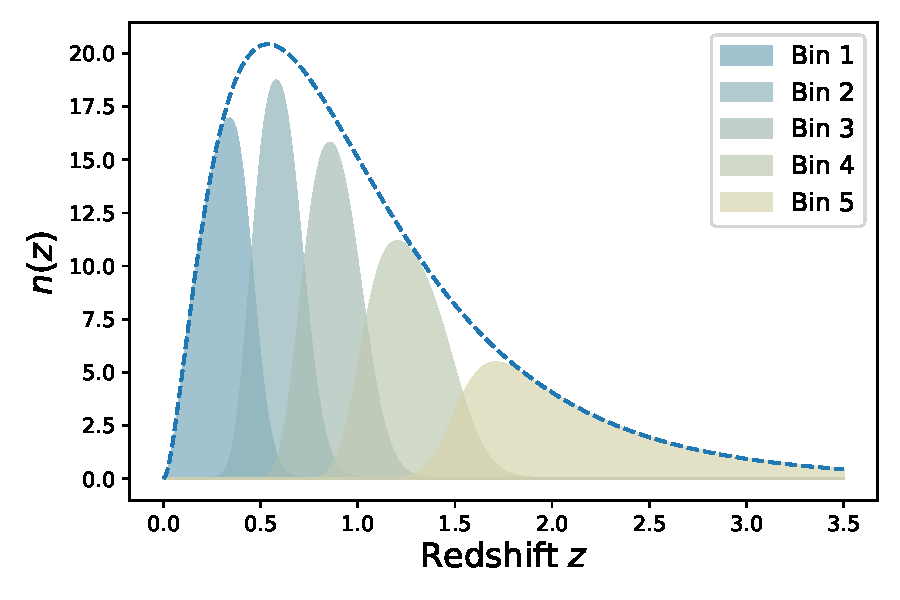
\includegraphics[width=\columnwidth]{figures/redshift_distribution_light.pdf}
    \caption{
     Source sample redshift distributions for each tomographic bin for LSST Y10. The number density on the y-axis is shown in arcmin$^2$.
    }
     \label{fig:redshift_distribution}
\end{figure}
%--------------------------------------------------------------------
%--------------------------------------------------------------------
%--------------------------------------------------------------------
%------------------------------------------------------------------
\section{Experiment}\label{Sec:experiment}
%--------------------------------------------------------------------
%--------------------------------------------------------------------
%--------------------------------------------------------------------
\subsection{Explicit Inference}
%--------------------------------------------------------------------
%--------------------------------------------------------------------
%--------------------------------------------------------------------
\subsubsection{Power spectrum}
%--------------------------------------------------------------------
%--------------------------------------------------------------------
%--------------------------------------------------------------------
To obtain the probability distribution of the cosmological parameters using a summary-statistics-methods, we focus on the 2-point statistics, specifically, on the angular power spectra $C_{\ell}$.
We assume a Gaussian likelihood with a cosmology-independent covariance matrix:
\begin{equation}
    \log{\mathcal{L}}(\bm{\theta})=-\frac{1}{2}[\bm{d}-\bm{\mu}(\bm{\theta})]^{T}\bm{C}^{-1}[\bm{d}-\bm{\mu}(\bm{\theta})].
\end{equation}
To compute the expected theoretical predictions $\bm{\mu}(\bm{\theta})$ we use the public library \href{https://github.com/DifferentiableUniverseInitiative/jax_cosmo}{\texttt{jax-cosmo}}. 
 The Covariance matrix $\bm{C}$ of the observables is computed at the fiducial cosmology, presented in \autoref{tab:prior}, using the same theoretical library. Specifically, in {\texttt{jax-cosmo}}, the Gaussian covariance matrix is defined as:
\begin{equation}
    \text{Cov}(C_{\ell},C_{\ell}')=\frac{1}{f_{sky}(2 \ell+1)}\left(C_{\ell}+\frac{\sigma_{\epsilon}^2}{2n_s}\right)
\end{equation}
where $f_{sky}$ is the fraction of sky observed by the survey, and $n_s$ is the number density of galaxies. 
To obtain the data vector $\bm{d}$, containing the auto- and the cross-power spectra for each tomographic bin, we use the \href{https://lenstools.readthedocs.io/en/latest/lenstool} {\texttt{LensTools}} package \citep{2016A&C....17...73P} on a single noisy simulated map (our fiducial).
%--------------------------------------------------------------------
%--------------------------------------------------------------------
%--------------------------------------------------------------------
\subsubsection{Full field with BHMs}
%--------------------------------------------------------------------
%--------------------------------------------------------------------
%--------------------------------------------------------------------
To construct the explicit map-based inference strategy in the Hierarchical Bayesian framework, we built a likelihood based on the data model described in \autoref{Sec:Lognormal Modeling}. 
As mentioned before, this means that the simulator serves as the physical deterministic model capable of generating the non-linear representation of the convergence map.

However, in practical terms, the measurement of convergence for each pixel and bins will differ from real observations due to noise. This is taken into consideration in the likelihood. Specifically, for LSST Y10, the number of galaxies for each pixel should be sufficiently high so that, according to the central limit theorem, we can assume the observation is characterized by Gaussian noise, with $\sigma_n^2=\sigma_e^2/N_s$, where $N_s$ represents the total number of source galaxies per bin and pixel. Given $\sigma_n^2$ the variance of this Gaussian likelihood, its log-form can be expressed as:
\begin{equation}
    \mathcal{L}(\bm{\theta})=
    \sum_i^{N_{pix}} \sum_{j}^{N_{bins}} \log{P(\kappa^{obs}_{i,j}|\kappa_{i,j},\bm{\theta})}
    =\sum_i^{N_{pix}} \sum_{j}^{N_{bins}}\frac{[\kappa_{i,j}-\kappa^{obs}_{i,j}]^2}{2\sigma_n^2},
\end{equation}
where $\kappa^{obs}$ refers to the values of convergence from noise maps. \\
Since the full-field approach does not rely on any summary statistics, it typically leads to a high-dimensional problem, requiring more sophisticated statistical techniques. To sample the posterior distribution for $\bm{\theta}$, we use a Hamiltonian Monte Carlo (HMC) algorithm. The HMC algorithm is particularly helpful in high-dimensional spaces where a large number of steps are required to effectively explore the space. It improves the sampling process by leveraging the information contained in the gradients to guide the sampling process. As the code is implemented in Jax, the gradients are accessible via automatic differentiation. 
%--------------------------------------------------------------------
%--------------------------------------------------------------------
%--------------------------------------------------------------------
\subsection{Implicit Inference}
%--------------------------------------------------------------------
%--------------------------------------------------------------------
%--------------------------------------------------------------------
\subsubsection{Benchmark compression scheme}
To ensure the scalability of density estimation LFI in cases where forward simulations are computationally expensive, it becomes necessary to employ compression techniques that reduce the dimensionality of the data space and extract summary statistics. 
Specifically, we try to find a function $\bm{t}=F(\bm{d})$, where $\bm{t}$ represents low-dimensional summaries of the original data vector $\bm{d}$. The objective is to achieve a compression function $F(\bm{d})$ that maximizes the information while minimizing dimensionality. Previous studies \citep{alsing2018generalized} have demonstrated that, under specific conditions, a compression scheme can be achieved where the dimension of the summaries dim($\bm{t}$) is equal to the dimension of the unknown parameters dim($\bm{\theta}$) without any loss of information at the Fisher level. Multiple approaches exist in an attempt to satisfy this condition. This section aims to provide an overview of the various neural compression-based methods employed in previous works.
%--------------------------------------------------------------------
\paragraph{\textcolor{violet}{Mean Square Error (MSE)}}
%--------------------------------------------------------------------
One of the commonly used techniques for training a Neural Network is by minimizing the $L_2$ norm or Mean Square Error (MSE).
This methods has been widely adopted in various previous studies  \citep{ribli2018improved, lu2022simultaneously, lu2023cosmological}, where the loss function is typically formulated as follows:
\begin{equation}
   \mathcal{L}=\frac{1}{N_{\theta}}(\bm{t}-\bm{\theta})^2.
\end{equation}
Here $N_{\theta}$ represents the number of cosmological parameters, $\bm{t}$ denotes the summary statistics, and $\bm{\theta}$ corresponds to the data vector of the cosmological parameters. 
However, it is important to note that this approach does not guarantee the recovery of maximally informative summary statistics. While this may hold true for fixed fiducial values of the cosmological parameters and assumptions of Gaussianity, its validation to more generic cases need to be proved. Indeed, minimizing the $L_{2}$ norm is equivalent to training the model to estimate the mean of the posterior distribution. We prove this statement in \autoref{Sec:appendix_Mean Square Error}.
%--------------------------------------------------------------------
\paragraph{\textcolor{violet}{Maximum Absolute Error (MAE)}}
%--------------------------------------------------------------------
Another commonly used approach involves minimizing the $L_1$ norm or Mean Absolute Error (MAE). In this approach, the loss function is defined as:
\begin{equation}
    \mathcal{L}=|\bm{t}-\bm{\theta}|
\end{equation}
where $\bm{t}$ represents the summary statistics and $\bm{\theta}$ denotes the cosmological parameters.
In \autoref{Sec:appendix_Maximum Absolute Error}, we demonstrate that minimizing this loss function is equivalent to training the model to estimate the median of the posterior distribution. While extensively employed in various previous studies \citep{2018PhRvD..97j3515G, fluri2018cosmological, ribli2019weak}, similar to the previous consideration for the MSE, it is important to note that the effectiveness of this loss function in extracting sufficient statistics needs to be demonstrated in more generic applications.
%--------------------------------------------------------------------
\paragraph{\textcolor{violet}{Variational Mutual Information Maximization (VMIM)}}
%--------------------------------------------------------------------
The Variational Mutual Information Maximization (VMIM) technique was first introduced for cosmological inference problems by \citet{jeffrey2021likelihood}. This approach aims to maximize the mutual information $I(\bm{t}, \bm {\theta})$ between the cosmological parameters $\bm{\theta}$ and the summary statistics $\bm{t}$.
In the VMIM approach, the loss function is defined as:
\begin{equation}\label{Eq:Loss_vmim}
    \mathcal{L}=- \log{q(\bm{\theta}|\bm{t};\bm{\varphi'})}.
\end{equation}
Here, $q(\bm{\theta}|\bm{t};\bm{\varphi'})$ represents a variational conditional distribution, $\bm{t}$ denotes the summary statistics, $\bm{\theta}$ corresponds to the data vector of the cosmological parameters, and $\bm{\varphi'}$ are the parameters of the Neural Network.
In order to understand the significance of this loss function, it is necessary to start by considering the mathematical definition of mutual information $I(\bm{t}, \bm {\theta})$:
\begin{align}\label{Eq:mutual_information}
    I(\bm{t}, \bm {\theta}) &= D_{KL}(p(\bm {t}, \bm {\theta})||p(\bm {t})p(\bm {\theta})) \\ \nonumber
    &= \int d^n \bm{\theta} d^n \bm{t} p(\bm t, \bm \theta)\log{\left( \frac{ p(\bm {t}, \bm {\theta})}{ p(\bm {t}) p(\bm {\theta})} \right)} \\ \nonumber
    &= \int d^n \bm{\theta} d^n \bm{t} p(\bm t, \bm {\theta})\log{\left( \frac{ p(\bm {\theta} | \bm {t} )}{ p(\bm {\theta})} \right)} \\ \nonumber
        &= \int d^n \bm{\theta} d^n \bm{t} p(\bm t, \bm {\theta})\log{p(\bm {\theta} | \bm {t} )} - \int d^n \bm{\theta}  d^n \bm{t} p(\bm t, \bm {\theta})\log{p(\bm {\theta})} \\ \nonumber
    &= \int d^n \bm{\theta} d^n \bm{t} p(\bm t, \bm {\theta})\log{p(\bm {\theta} | \bm {t} )} - \int d^n \bm{\theta} p(\bm {\theta})\log{p(\bm {\theta})} \\ \nonumber
    &= \mathbb{E}_{p(\bm {t}, \bm {\theta})} [\log{p(\bm {\theta} | \bm {t} )}]- \mathbb{E}_{p(\bm {\theta})} [\log{p(\bm {\theta})}] \\ \nonumber
    &= \mathbb{E}_{p(\bm {t}, \bm {\theta})} [\log{p(\bm {\theta} | \bm {t} )}]- H(\bm {\theta});
\end{align}

in the above equation, $D_{KL}$ is the Kullback-Leibler divergence \citep{kullback1951information}, $p(\bm {t}, \bm {\theta})$ is the joint probability distribution of summary statistics and cosmological parameters, and $H(\bm {\theta})$ represents the \textit{entropy} of the distribution of cosmological parameters.  
Essentially, mutual information measures the amount of information contained in the summary statistics $\bm t$ about the cosmological parameters $\bm \theta$. The summary statistics $\bm{t}$ are extracted from the original high-dimensional data vector $\bm{d}$ using $\bm{t}=F_{\bm {\varphi}}(\bm{d})$.
The goal is to find the parameters $\bm {\varphi}$ that maximize the mutual information between the summary and cosmological parameters:
\begin{equation}
   \bm {\varphi}^*= \operatorname*{argmax}_{\bm {\varphi}} I(F_{\bm {\varphi}}(\bm{d}), \bm {\theta}).
\end{equation}
However, the mutual information expressed in \autoref{Eq:mutual_information} is not tractable. To overcome this limitation, various approaches have been developed that rely on tractable bounds, enabling the training of deep neural networks to optimize the mutual information. In this study, we adopt the same strategy used by \citet{jeffrey2021likelihood}, which involves using the variational lower bound \citep{barber2003information}:
\begin{equation}\label{Eq:variational_lower_bound}
    I(\bm{t}, \bm{\theta}) \ge \mathbb{E}_{p(\bm {t}, \bm {\theta})} [\log{q(\bm {\theta} |\bm{t} ; \bm{\varphi}')}]- H(\bm {\theta}).
\end{equation}
Here, the variational conditional distribution $\log{q(\bm {\theta} |\bm{t}; \bm{\varphi}')}$ is introduced to approximate the true posterior distribution $p(\bm{\theta}|\bm {t})$. 
As the entropy of the cosmological parameters remains constant for a fixed training set, the optimization problem based on the lower bound in \autoref{Eq:variational_lower_bound} can be formulated as:
\begin{equation}
    \operatorname*{argmax}_{\bm {\varphi}, \bm {\varphi}'}\mathbb{E}_{p(\bm {d}, \bm {\theta})} [\log{q(\bm {\theta} |F_{\bm {\varphi}}(\bm {d}) ; \bm{\varphi}')}], 
\end{equation}
yielding \autoref{Eq:Loss_vmim}.
%--------------------------------------------------------------------
\paragraph{\textcolor{violet}{Gaussian Negative Log-Likelihood (GNLL)}}
%--------------------------------------------------------------------
\FL{Recognizing that the uncertainty on different cosmological parameters will vary, a third
class of inverse variance weighted MSE was proposed in \cite{fluri2018cosmological} with the idea of
ensuring that each parameter contributes fairly to the overall loss by taking into account its uncertainty. The loss function typically takes the following form:
\begin{equation}
    \mathcal{L} = \frac{1}{2} \log(|\Sigma|) + \frac{1}{2}(t - \theta)^t \Sigma^{-1} (t - \theta) 
\end{equation}
where $t$ is the summary statistics and $\Sigma$ is the covariance matrix of representing the uncertainty on the cosmological parameters $\theta$. Both $t$ and $\Sigma$ can be outputs of the compression network, i.e. $f_\theta(x)=(t, \Sigma)$.

One recognizes here the expression of a Gaussian probability function, and this expression can thus be straightforwardly related to the VMIM case by simply assuming a Gaussian distribution as the variational approximation for the posterior $q(\theta | x) = \mathcal{N}(\theta; t, \Sigma)$.

This means that this loss function is actually sub-optimal for two reasons:
\begin{itemize}
    \item The summary extracted by the neural network $t$ is, similarly to the MSE case only an estimate of the mean of 
    the posterior distribution, which is not guaranteed to be sufficient.
    \item Because of the Gaussian variational assumption, the variational posterior can potentially be biased with respect to the true posterior, and thus the mean of this Gaussian approximation may be biased with respect to the true posterior mean.
\end{itemize}
 A simple MSE would thus seem to be preferable.
}
%--------------------------------------------------------------------
\paragraph{\textcolor{violet}
{Information Maximising Neural Networks (IMNNs)}}. \LM{TODO: condensed introduction; emphasize learning compression at single point; network learns score function which generalises smoothly away from fiducial \cite{Makinen_2021, Makinen_2022, Charnock_2018}, Wandelt (in prep.) 
}
%--------------------------------------------------------------------
\subsection{Compression strategy}
%--------------------------------------------------------------------
We aim to examine the impact of different loss functions used to train the compressor on the final cosmological constraints. We employ the same convolutional neural network architecture to build the compressor. Specifically, we utilize a deep ResNet architecture \citep{he2016deep}, the ResNet-18, implemented using Haiku \citep{haiku2020github}, a Python deep learning library built on top of JAX. While the different compression strategies share the same architecture, the training strategies for VMIM and GNLL differ significantly. To train the Neural compressor under VMIM and GNLL, we jointly optimize the weights of the Neural Network $F_{\varphi}$ (the compressor) and the parameters of the variational distribution $q_{\varphi'}$. For VMIM, the variational distribution $q(\bm{\theta}|\bm{t};\varphi')$ is modeled using a Normalizing Flow, while for GNLL, a Conditional Multivariate Gaussian estimator is employed. The Normalizing Flow used for the inference strategy is also adopted for the variational distribution required in the compression procedure. For the Multivariate Gaussian estimator, we implement a three-layer neural network. The first two layers consist of fully connected layers with a Leaky Rectified Linear Unit activation function and a hyperbolic tangent activation function, respectively. The number of channels is increased to 256 and 128 for the first two layers, respectively. The last layer is a fully connected layer without an activation function, responsible for mapping the output of the first two layers to the desired output size (mean and covariance of the Gaussian distribution).
%--------------------------------------------------------------------
%--------------------------------------------------------------------
%--------------------------------------------------------------------
%--------------------------------------------------------------------
\subsubsection{Inference strategy}\label{Sec:Inference_strategy}
%--------------------------------------------------------------------
%--------------------------------------------------------------------
By comparing the posteriors $p(\theta| t)$ obtained with different compression strategies, we can assess the sensitivity of the results to the choice of statistics. In particular, the more informative the summary statistics, the “closer” the posterior $p(\theta | t)$ is to the true posterior $p(\theta | x)$. In this section, we describe how we approximate the posterior distribution for each summary statistic t, enable us to use it as a fair benchmark for comparison (we describe the performance metric in section ??).\\
Since the likelihood $p(t|\theta)$ is intractable, we propose to do Neural Posterior Estimation \citep{npe1, npe2, npe3}, a Simulation-Based Inference (SBI) strategy that aims to directly approximate, from simulations, the posterior distribution 
\begin{equation}
    p(\theta | t) \propto \int p(t | \theta, z) p(z|\theta) p(\theta) dz\,.
\end{equation}

Usually, NPE algorithm approximates the posterior distribution through the use of conditional Normalizing Flows $p_{\varphi} (\theta | t)$ \citep{nf1, nf2}. This is achieved by minimizing the negative log probability: 

\begin{equation}
    \mathbb{E}_{p(\theta, t)} \left[ - \log p_{\varphi} (\theta | t)  \right].
    \label{eq:nll}
\end{equation}

Finally, the target posterior $p(\theta | t = t_0)$ is approximated by $p_{\varphi}(\theta | t = t_0)$ where $t_0 = t(x_0)$ with $x_0$ the observed convergence map.

For each summary statistic, we approximate it posterior distribution using the same NF architecture, namely a RealNVP \citep{realnvp} with 4 coupling layers, shift and scale parameters are learned using a neural network with 2 layers of 128 neurons, activation functions are $silu$ \citep{silu}. And, for each summary statistic, the prior $p(\theta)$ used in the inference process remains the same.
%--------------------------------------------------------------------
%--------------------------------------------------------------------
\subsection{Result estimators}
%--------------------------------------------------------------------
%--------------------------------------------------------------------
To evaluate the results obtained from different approaches, we use two commonly employed estimators found in the literature. Their definitions are provided in the following sections.
%--------------------------------------------------------------------
\subsubsection{Figure of Merit (FoM)}
%--------------------------------------------------------------------
To quantify the constraining power of each inference strategy, we first employ the Figure of Merit (FoM), defined as follows:
\begin{equation}\label{Eq:Figure_of_merit}
    \text{FoM}_{\alpha \beta}=\sqrt{\text{det}(\Tilde{F}_{\alpha \beta})}.
\end{equation}
Here, $\alpha$ and $\beta$ represent a pair of cosmological parameters, and $\Tilde{F}_{\alpha \beta}$ refers to the marginalized Fisher matrix. We calculate $\Tilde{F}_{\alpha \beta}$ as the inverse of the parameter space covariance matrix $C_{\alpha \beta}$, which is estimated from the HMC chains and from the Normalizing flow sampling. 
Under the assumption of a Gaussian covariance, the FoM defined in \autoref{Eq:Figure_of_merit} is proportional to the inverse of the $2-\sigma$ contours in the 2-dimensional marginalised parameter space of the $\alpha$ and $\beta$ pair.
%--------------------------------------------------------------------
\subsubsection{Kullback-Leibler divergence}
%--------------------------------------------------------------------
To measure the difference between the probability distribution obtained with different compressed summaries we compute the \textit{Kullback-Leibler divergence} or KL-divergence. As mentioned when we introduced the VMIM, the KL divergence is related to the relative entropy, and is a non-symmetric measure of the difference between two distributions. \denise{INCOMPLETE}
%--------------------------------------------------------------------
% ############# Begin Table BiblioSruvey  #############
%--------------------------------------------------------------------
\begin{table*}
    \begin{center}
        \begin{tabular}{ |p{3.5cm}|p{3.5cm}|p{3.5cm}|p{4cm}|  }
            \hline
            Reference &  \makecell{Loss function} & \makecell{Inference \\ strategy} & \makecell{Output compressor}   \\
            \hline
            \citet{2018PhRvD..97j3515G} & \makecell{MAE} &  \makecell{Likelihood \\ analysis} &\makecell{$\sigma_8, \Omega_m$}  \\
            \hline
            \citet{fluri2018cosmological} & \makecell{GNLL} & \makecell{Likelihood \\ analysis} &  \makecell{$\log{(\sigma_{\Omega_m}^2)},\log{(\sigma_{\sigma_8}^2)}$,
             \\
            $\tanh^{-1}{(\text{Corr}(\sigma_8,\Omega_m))}$,
             \\
            $\sigma_8,\Omega_m$} 
            \\
            \hline     
            \rowcolor{lightgray}
                        \citet{fluri2019cosmological} &  \makecell{GNLL} & \makecell{Likelihood \\ analysis} & \makecell{$\sigma_8, \Omega_m, A_{IA}/10, L$  \\ with  $L:\Sigma^{-1}=LL^{T}$}
            \\
            \hline            
                        \citet{ribli2018improved} & \makecell{MSE}  &\makecell{RMSE for \\ evaluation}  & \makecell{$\sigma_8, \Omega_m$}   
            \\
            \hline            
                        \citet{ribli2019weak} & \makecell{MAE} & \makecell{Likelihood \\ analysis} & \makecell{$\sigma_8, \Omega_m$}   
            \\            
            \hline             
                        \citet{PhysRevD.102.123506} & \makecell{MAE} & \makecell{Likelihood \\ analysis} & \makecell{$\sigma_8, \Omega_m$}   
            \\
            \hline 
            \rowcolor{lightgray}
                        \citet{jeffrey2021likelihood} & 
                        \makecell{MSE \\ VMIM}
                        & \makecell{PyDelfi} & \makecell{$\varphi: F_{\varphi}(\bm{d})=\bm{\theta}$ \\ with $\bm{\theta}=\Omega_m, \sigma_8$}    
            \\            
            \hline             
                        \citet{fluri2021cosmological} &\makecell{FIM} & \makecell{GPABC} &  
            \\
            \hline      
            \rowcolor{lightgray}
            
                        \citet{fluri2022full} &  \makecell{FIM} & \makecell{GPABC} &  
            \\            
            \hline 
                        \citet{lu2022simultaneously} & \makecell{MSE} & \makecell{Likelihood \\ analysis}  & \makecell{$\Omega_m,S_8, A_{IA}/10,$ \\ rescaled \\ baryonic parameters \\ $(M_c,M_{1,0}, \eta, \beta)$}   
            \\           
            \hline 
                        \citet{kacprzak2022deeplss} & \makecell{GNLL}  & \makecell{Likelihood \\ analysis}  & \makecell{WL: $\Sigma, \Omega_m, \sigma_8, A_{IA}, \eta_{IA}$ \\  GC:$\Sigma, \Omega_m, \sigma_8, b_g, r_g,\eta_{b_{g}}$ }
                      
            \\
            \hline 
            \rowcolor{lightgray}
                        \citet{lu2023cosmological} &  \makecell{MSE} & \makecell{Likelihood \\ analysis}  & \makecell{$\Omega_m,S_8,A_{IA}/10,$\\ rescaled baryonic \\ parameters: $M_c,M_{1,0}, \eta, \beta$} 
        \end{tabular}
        \caption{Table summarizing the current state of the art for neural compression schemes. The table includes all studies conducted within the context of Implicit analysis and standard Likelihood analysis. The shaded gray region indicates analyses performed on real observations. \\ 
        Abbreviations used in the Table: MSE-Mean Square Error; MAE-Maximum Absolute Error; GNLL- Gaussian Negative Log Likelihood; VMIM- Variational Mutual Information Maximization; FIM- Fisher Information Matrix; GPABC-Gaussian Processes Approximate Bayesian Computation. WL- Weak Lensing; GC-Galaxy Cluster.}
        \label{tab:biblio_survey}
    \end{center}
\end{table*}
%--------------------------------------------------------------------
% ############# End Table BiblioSruvey  #############
%--------------------------------------------------------------------
%--------------------------------------------------------------------
\section{Results}\label{Sec:results}
%--------------------------------------------------------------------
We present the results of the constraints on the full $\Lambda$CDM parameter space expected for a survey like LSST-Y10. The forecasted results are obtained using the simulation procedure outlined in \autoref{Sec:the SBILens framework} and the parameter inference strategy described in \autoref{Sec:Inference_strategy}.
We begin by analyzing the impact of the different compression strategies on the final cosmological constraints. Subsequently, we compare the outcomes of three different inference procedures: the 2-point statistics, the explicit full-field statistics, and the implicit full-field statistics using CNN summaries.
%--------------------------------------------------------------------
\subsection{Optimal compression strategy}
Figure X shows the posterior contours from one fiducial map using the compressed summaries.
%--------------------------------------------------------------------
\subsection{Power spectrum and full-field statistics}
%--------------------------------------------------------------------
We now compare the constraining power of the three different approaches described in \autoref{Sec:experiment}: the standard-two point statistics and two map-based approaches, the explicit inference using an HMC and the implicit inference using the Normalizing Flow as an estimator. 
As outlined before, our primary interest is to prove that the two map-based approaches lead to very comparable posterior distributions. We present the $68.3\%$ and $95.5\%$ confident regions for the full $\Lambda$CDM parameters in \autoref{fig:contours_posterior_imp_ex_ps}. The contours obtained by the angular $C_{\ell}$ analysis are plotted in blue, the ones for the HMC in yellow, and those for the Normalizing Flow in violet. 
We can see from the figure that the contours from the HMC-based inference and the Normalizing flow-based inference are remarkably similar.  We quantify the results by computing the Figure of Merit as described in \autoref{Eq:Figure_of_merit}. The results are presented in \autoref{tab:f_o_m}. The
The remarkably strong agreement between the two posteriors confirms that the two map-based cosmology inference methods yield the same results. This establishes the validity of the implicit inference strategy.
Moreover, we find that the two-point statistic is suboptimal in constraining $\Omega_c$, $\sigma_8$, and $w_0$, while the two map-based approaches yield much tighter constraints on these parameters. Additionally, for the full-field strategies we find that the size of the contours is significantly smaller than the size for the prior distributions adopted, suggesting that the 
posterior on these parameters are not affected by the specific choice of prior.
Confirming previous work, we note that $h$, $\Omega_b$, and $n_s$ result prior dominated and hence are constrained by none of the three approaches. 
We find that the map-based explicit and implicit strategies lead to an improvement in the figure of merit of 2.06, 1.98, 2.28 and 2.06, 1.90, 2.22, respectively, in the $\Omega_c-\sigma_8; \Omega_c-w_0; \sigma_8-w_0$ plane.

%--------------------------------------------------------------------
%--------------------------------------------------------------------
% ############# PLOT CONTOURS HMC-SBI-PS  #############
%--------------------------------------------------------------------
\begin{figure*}
    \centering
        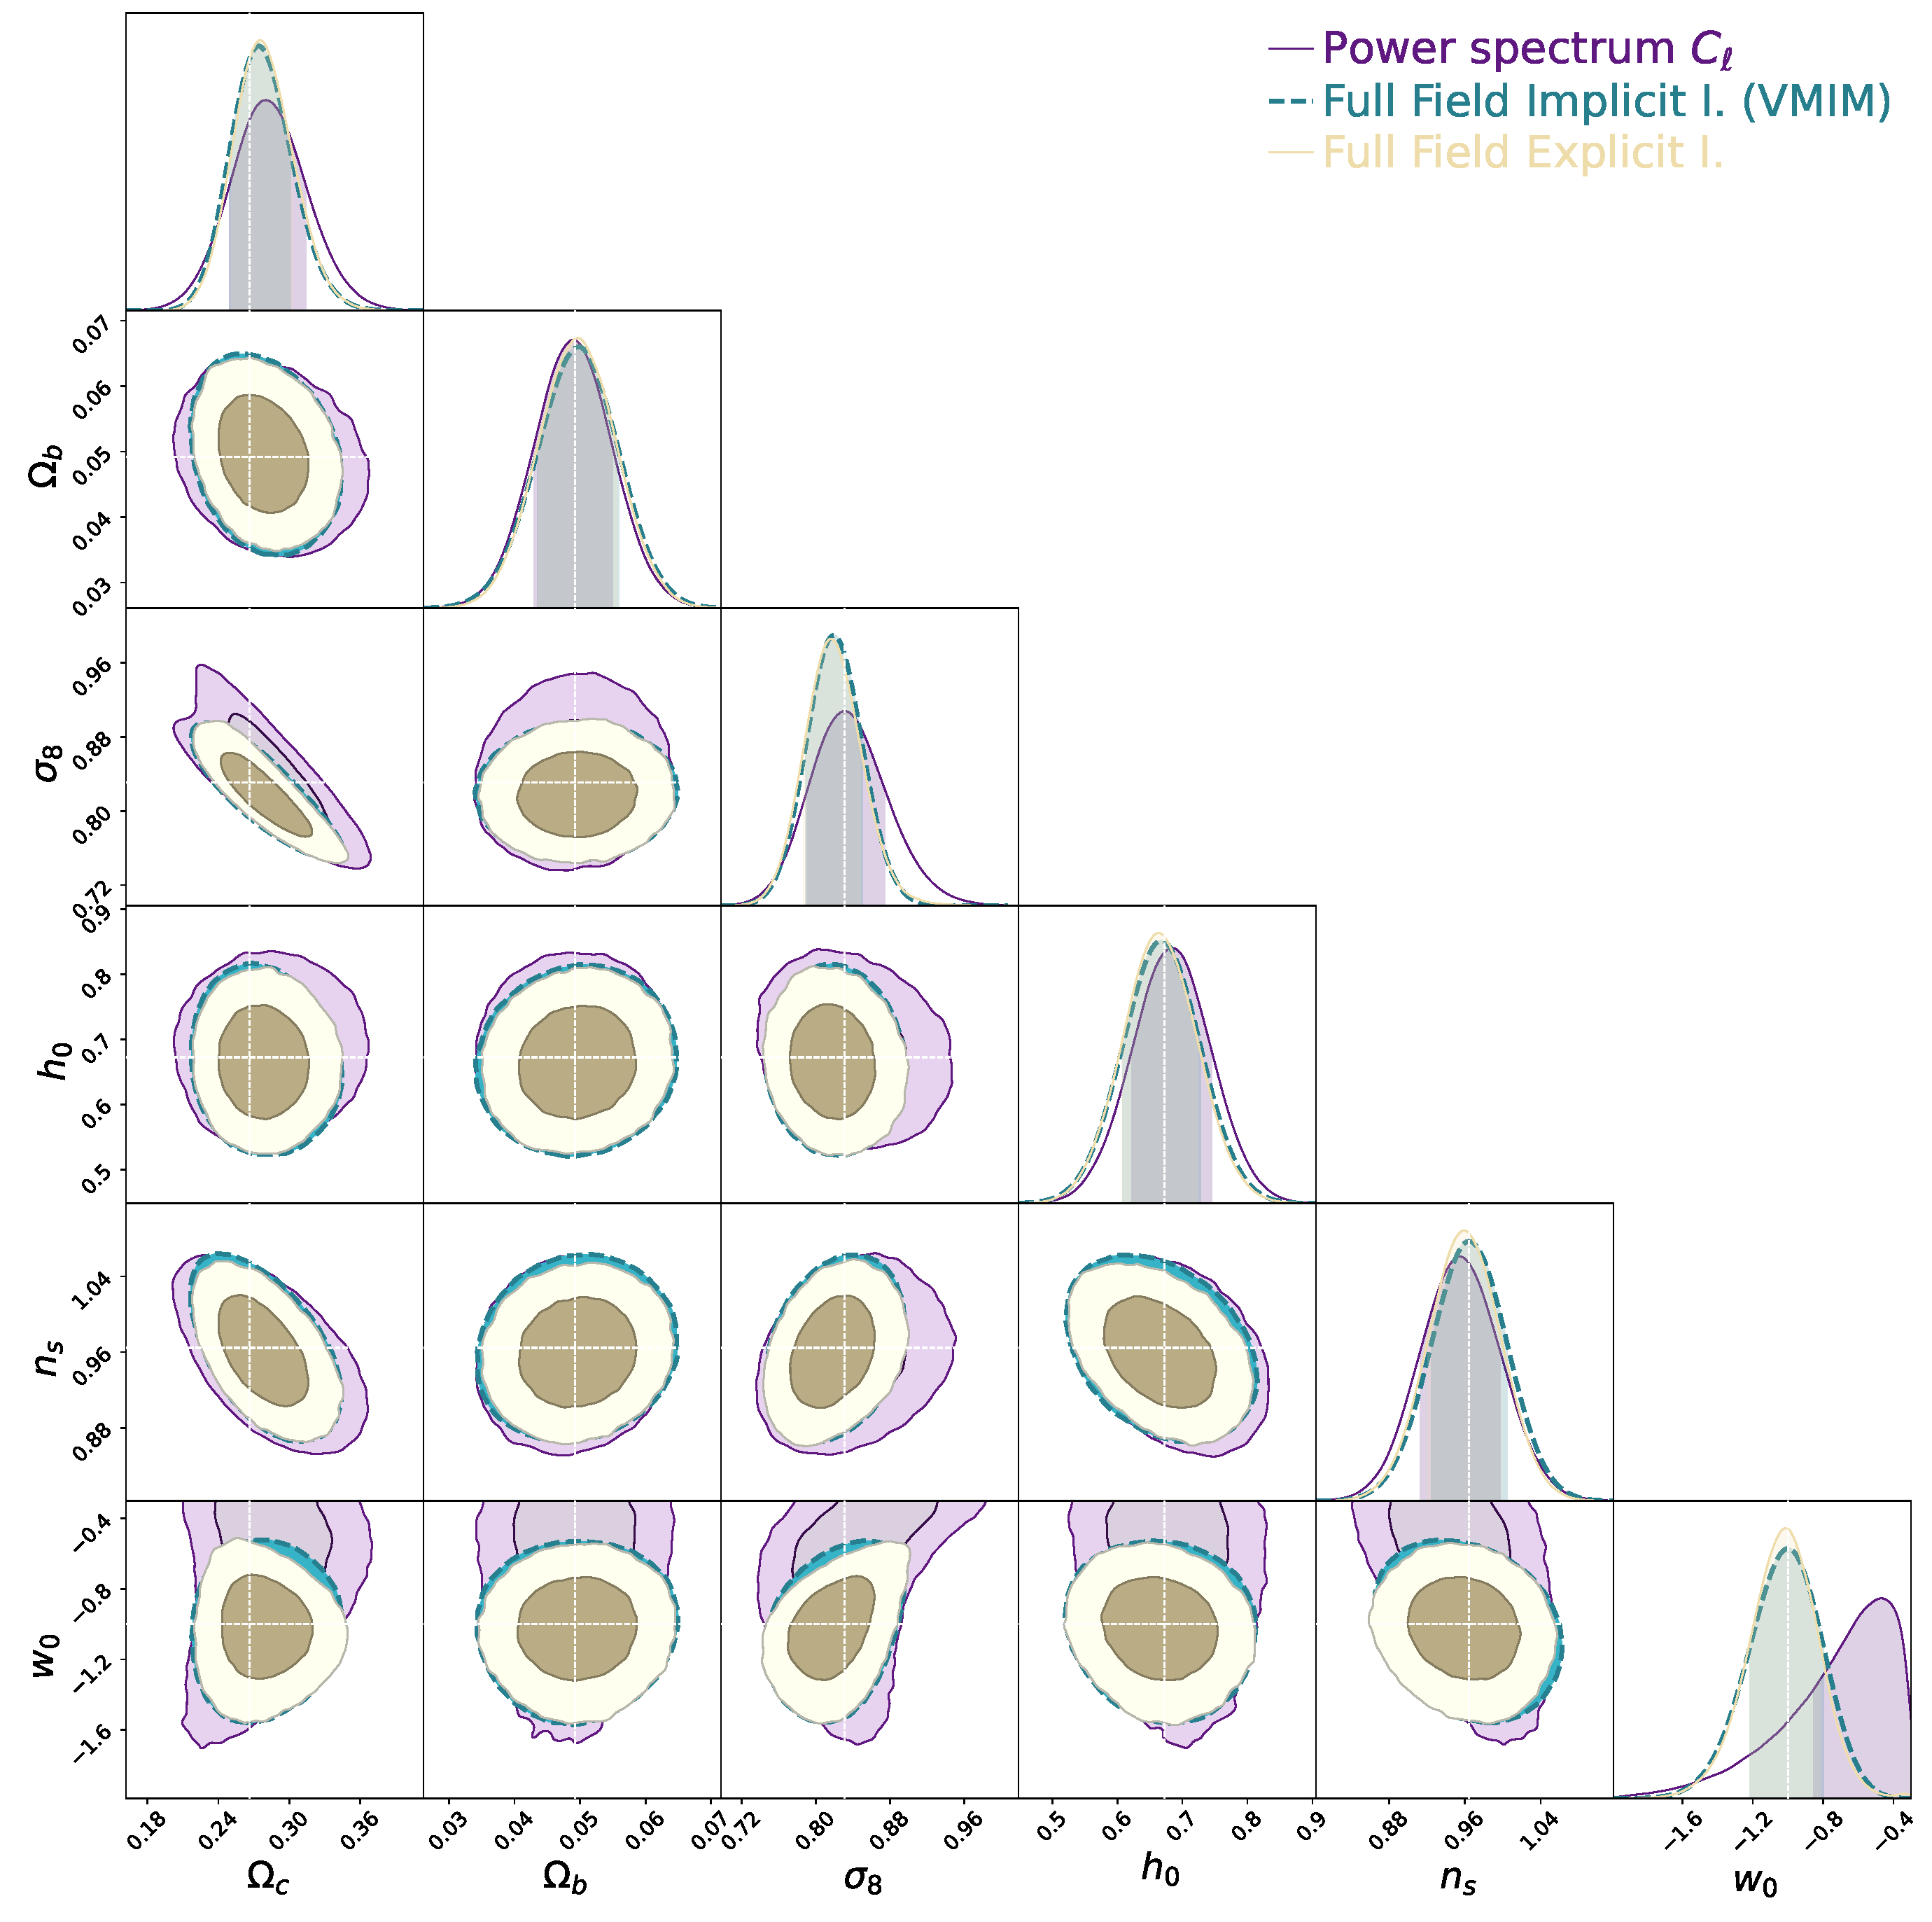
\includegraphics[width=\textwidth]{figures/contours_posterior_imp_ex_ps.pdf}
        \caption{
        Constraints on the $\Lambda$CDM parameter space as found in the LSST Y10 survey setup. The constraints are obtained by applying the $C_{\ell}$ (light blue contours), the full field explicit inference (yellow contours), and the full field implicit inference strategy (violet contours), described in \autoref{Sec:experiment}.
        The contours show the $68\%$ and the $95\%$  confidence regions. The dashed white lines define the true parameter values.}
        \label{fig:contours_posterior_imp_ex_ps}
\end{figure*}
%--------------------------------------------------------------------
% ############# FIGURE OF MERIT TABLE  #############
%--------------------------------------------------------------------
\begin{table*}
    \begin{center}
        \begin{tabular}{lcccccc} 
            \hline
            FoM & $C_{\ell}$ & Full Field (HMC)&  VMIM & MSE & MAE & GNLL   \\
            \hline\hline
            $\Omega_c-  \sigma_8$ & 1222 & 2520 & 2526 & 2043 & 2316\\
            $\Omega_c-  w_0$      & 100  & 198  & 190  & 152  & 162\\
            $\sigma_8-  w_0$      & 77   & 176  & 171  & 139  & 149\\
            \hline
        \end{tabular}
        \caption{ Values of the Figure of Merit (FoM) as defined in \autoref{Eq:Figure_of_merit} for different inference strategies: the convergence power spectrum $C_{\ell}$, the HMC, the CNN map compressed statistics with the MSE, the VMIM, the MAE and the GNLL loss functions. The values of the figure of merit are inversely proportional to the area of the contours, larger the FoM, higher the constraining power.}
        \label{tab:f_o_m}
    \end{center}
\end{table*}
%--------------------------------------------------------------------
%  ############# SUMMARY TABLE  #############
%--------------------------------------------------------------------
\begin{table*}
    \begin{center}
        \begin{tabular}{|l|l|l|l|l|l|l|l|l|}
            \hline
            \multirow{2}{*}{} &
            \multicolumn{2}{c|}{VMIM} &
            \multicolumn{2}{c|}{MSE} &
            \multicolumn{2}{c|}{MAE} &
            \multicolumn{2}{c|}{GNLL} \\
            & Mean & $\sigma$ & Mean & $\sigma$ & Mean & $\sigma$  & Mean & $\sigma$ \\
            \hline
            \hline
            $\Omega_c$ & 0.2742 & 0.026 & 0.2830 & 0.030 & 0.2793 & 0.029  & 2.1\% & 2.1\%\\
            \hline
            $\Omega_b$ & 0.0499 & 0.006 & 0.0492 & 0.006 &  0.0501 & 0.006 & 2.1\% & 2.1\% \\
            \hline
            $\sigma_8$ & 0.819 & 0.03 &0.808 & 0.03 &  0.808 &0.03 & 2.1\% & 2.1\% \\
            \hline
            $w_0$      &-0.998 & 0.2 &-1.13 & 0.2 & -1.16& 0.2  & 2.1\% & 2.1\% \\
            \hline
            $h_0$      & 0.6658 & 0.058 &0.6620 & 0.057 & 0.6640 & 0.057&  2.1\% & 2.1\% \\
            \hline
            $n_s$      & 0.9635 & 0.04 & 0.9559 & 0.04 & 0.9547 & 0.04  & 2.1\% & 2.1\% \\
            \hline
        \end{tabular}
        \caption{Marginalised mean and standard deviation of the parameter distributions.}
  \end{center}
\end{table*}
%--------------------------------------------------------------------
%--------------------------------------------------------------------
\section{Summary and conclusions}\label{Sec:conclusion}
 In this work, we presented and compared two different map-based strategies for inferring cosmological parameters: the explicit full-field strategy, also known as Bayesian Hierarchical inference, based on an HMC sampler, and the implicit inference strategy, also known as Likelihood-Free Inference. \\Deep learning approaches for implicit inference typically involve two steps: the automatic learning of an optimal low-dimensional summary statistic and the use of a Neural Density Estimator in low dimensions to either build an estimate $P_{\varphi}$ of the likelihood function $p(x|\theta)$ (Neural Likelihood Estimation) or build an estimate $P_{\varphi}$ of the posterior distribution $p(\theta|x)$ (Neural Posterior Estimation).
 
 The primary goal of this paper was to find an optimal compression strategy and demonstrate that, by using this strategy, both implicit and explicit methods yield the same posterior. \\
To both forward model the convergence maps and simulate the mock data used to train the implicit model, we developed \href{https://github.com/DifferentiableUniverseInitiative/sbi_lens}{\url{SbiLens}}, a Jax-based weak lensing simulator optimized for inference applications requiring access to the derivatives of the model. Our analysis is based on synthetic weak lensing data with five tomographic bins for a survey like LSST-Y10. \\
We begin by providing an overview of the different compression strategies adopted in the literature for both Likelihood-Free Inference and likelihood-based inference strategies. We then compare the impact of these different loss functions on the final constraints on the cosmological parameters for a $\Lambda$CDM model. 
We found the following results:
\begin{enumerate}
    \item The Mean Square Error and the Maximum Absolute Error lead to significantly similar results, while the VMIM (Variational-Mutual Information Maximization) leads to noticeably different contours, especially for the $w_0$ parameter. We quantified these differences by examining the figure of merit, standard deviation, and mean of the contours, and found that, although not substantial, the VMIM produces better results in terms of contour width and alignment with the fiducial value(??).
    \item  When using the VMIM to compress the original high-dimensional data, we compared the posterior obtained in the implicit inference framework with those obtained from Bayesian hierarchical modeling and power spectrum. We demonstrate that both map-based approaches lead to a significant improvement in constraining $\Omega_c, w_0, \sigma_8$ compared to the 2-point statistics. However, $h, n_s,\Omega_b$ are not constrained by either and are prior dominated.
    \item   When using the VMIM to compress the original high-dimensional data,  in the limit of our setting, the two methods, i.e. the Bayesian hierarchical inference and the Likelihood free inference, leads to the same posterior distributions.  
\end{enumerate}

It is important to discuss the limitations of the methodology used in this paper and highlight particular strategies for future extensions and applications. In this work, we employed a physical model based on a lognormal prior, notoriously faster than simulation-based methods. Although we have shown that this description is sufficiently complex for our tasks, as evidenced by the different contours obtained from the full-field and power spectrum methods, it is important to note that this is a good approximation for the convergence at intermediate scales, but can not be appropriate to analyze small scales. 
For example, the lognormal shift parameters are computed using the \texttt{Cosmomentum} code \citep{friedrich2018density, friedrich2020primordial}, which employs perturbation theory. However, as mentioned by \citet{boruah2022map}, the perturbation theory-based approach may not provide accurate results at small scales.
However, as the main objective of this paper was to compare the different inference strategies, we are not concerned with the potential implications of this approximation. In future applications, the simulation procedure will be based on N-body simulations.

Additionally, we did not include any systemic in the current application, although previous studies demonstrated that the map-based approaches help to dramatically improve the constraints on systematic and cosmological parameters in the presence of these last. The main reason for this absence is mainly related to the difficulty of modeling systematic effects, like for example intrinsic alignment, in the lognormal description. 

Hence, the natural next step will be to use N-body simulations as the physical model for the  \texttt{SBILens} package. Specifically, we aim to start from the model presented in [reference], and further develop it by including additional systematics such as the redshift uncertainties, the baryonic feedback, and a more complicated intrinsic alignment model. 
With these improvements, our model will be better suited to handle real cosmic shear data, allowing us to fully maximize the information gained from next-generation surveys.
 
%--------------------------------------------------------------------
%--------------------------------------------------------------------
\begin{acknowledgements}
This work was granted access to the HPC/AI resources of IDRIS under the allocation 2022-AD011013922 made by GENCI.
\end{acknowledgements}
%--------------------------------------------------------------------
%              #########    START BIBLIO   #########
%--------------------------------------------------------------------
\bibliographystyle{aa} % style aa.bst
\bibliography{paper/biblio} 
%--------------------------------------------------------------------
%--------------------------------------------------------------------

\textbf{Comments:}
\vspace{5mm}

\begin{itemize}
    \item \justine{Regarding the table with the differents losses - \citet{2018PhRvD..97j3515G} also used weighted MAE: 'Errors in predictions for maps from cosmologies in sparsely sampled regions are more severely penalized than those for maps from densely sampled re- gions. We show in §IV C that such a weighted loss func- tion reduces the bias in the predictions, at the cost of a longer network training, but has only a limited impact on the parameter constraints inferred from the predictions.'
    I think it's because they don't have honmogeneous dataset so if needed we can added a note to say that we are in the case of homogeneous dataset and thus don't have bias coming from this etc.
    + for inference startegy maybe we can say that It's gaussian likelihood with fixed cov matrix (evaluated at the fiducials) analysis.
    \item \citet{fluri2018cosmological} I think they use gaussian log likelihood loss where they learn both the mean and cov matrix: 'Similar to [26], we chose a negative log-likelihood loss as cost function' page 5. + because of bias issues they add regularization term at some point in the training.
    Then for the inference part they use a gaussian likelihood with mean and covariance matrix como dependent based on their CNN predictions.}
    \denise{yes, the use gnll, it was just a typo. 
However, they do not use the covariance matrix from the CNN predictions "
We did not use the network predictions of the covariance matrices for our main analysis. One reason was that
our examined test region was consisting out of four independent patches and the input of the network was only
one patch at a tim"} 
\justine{Yes you're right! They still present the case where you can use the covariance matrix, I mean in some way they try to pay attention to it.  Idk if you plan to describe a bit this table, if yes I think you can say that they propose this but end up just using the mean which is the exact same as doing mse etc... ?}
\denise{yep yep, the table is only a draft, and I didn't mention it in the paper yet. I will definitely describe it in more detail. Ps, sorry for the re-writing, I have OCD with latex error message}
\justine{yes ok no problem :) I was just checking the table since I'm currently reading these papers for our second project and did not know where to make these comments haha}
\LM{Ok sweet I was confused about this -- Fluri et al talk about this loss function (which I'm using in another project ahaha) but if they don't make use of the network Covariance it's just a weirdly-weighted MSE (also I wasn't convinced about their training routine in that paper -- the losses didn't seem converged)}
\item \justine{\cite{fluri2021cosmological} From my understanding, what they use is not exactly the imnn in the sense that they don't rely on gaussian assumptions for the summary distribution.}
\item \LM{Nope they don't use IMNN. They're using a regression-gnll loss, but they don't show any optimality guarantees using this form. Plus, they don't make use of the covariance in a particularly smart way (e.g. to reweight summary distributions for posterior construction) so it's not super useful. I'll be sure to explicitly show the difference in Fluri et al and the IMNN in the corresponding section.} \\
\justine{Awesome, thanks! :)}
\end{itemize}
\denise{I wrote IMNN for \cite{fluri2021cosmological} because their optimization, as for the IMNN, is based on the CramerRao bound, so on the Fisher Information. The difference is that in the IMNN there is an assumption of Gaussian distribution, which allows you to write the Fisher matrix as:
\begin{equation}
      F_{\alpha \beta}= \sum_{ij}\frac{\partial \mu}{\partial \theta_{\alpha}} C_{ij}^{-1}
      \frac{\partial \mu}{\partial \theta_{\beta}}
      \label{Fisher_matrix}
\end{equation}
and then the determinant of the fisher matrix is optimized.
In \cite{fluri2021cosmological} they minimize the determinant of the jacobian of the summaries and the determinant of the covariance. 
Both methods come from the CramerRao bound, but as Lucas said, this is something that has to be explained in the section. I could not write all of this in the Table. We can think of an acronym (FIM maybe? Fisher Information Matrix ) and introduce it in the proper section. 
}

%--------------------------------------------------------------------
%              #########    START APPENDIX   #########
%--------------------------------------------------------------------
\begin{appendix}
\section{Mean Square Error (MSE)}\label{Sec:appendix_Mean Square Error}
In this section, we demonstrate that minimizing the $L_2$ norm is equivalent to training the model to estimate the mean of the posterior distribution, namely:
\begin{equation}\label{Eq:mean_mse}
\left \langle \bm {\theta} \right \rangle_{p(\bm {\theta}|\bm{d})}=\operatorname*{argmin}_{\mathcal{F}(\bm{d})}\mathbb{E}_{p(\bm {\theta}|\bm {d})}[\left\Vert \bm {\theta}-\mathcal{F}(\bm{d})
 \right \Vert_{2}^{2}].
\end{equation}
To demonstrate \autoref{Eq:mean_mse}, we need to minimize the expected value of the $L_2$ norm with respect to $\mathcal{F}(\bm{d})$. Let us consider its derivative:
\begin{align}\label{Eq:moment_1}
   & \frac{\partial}{\partial \mathcal{F}(\bm{d}) }  \mathbb{E}_{p(\bm {\theta}|\bm{d}))}[(\bm {\theta}-\mathcal{F}(\bm{d}))^2] =  \\
    &
    \frac{\partial}{\partial \mathcal{F}(\bm{d}) }  \mathbb{E}_{p(\bm {\theta}|\bm {d})}[\bm {\theta}^2+\mathcal{F}(\bm{d})^2-2\bm {\theta}\mathcal{F}(\bm{d})] = \nonumber \\
    &
    \frac{\partial}{\partial \mathcal{F}(\bm{d}) }  [
    \mathbb{E}_{p(\bm {\theta}|\bm {d})}[\bm {\theta}^2]+\mathcal{F}(\bm{d})^2-2\mathcal{F}(\bm{d})\mathbb{E}_{p(\bm {\theta}|\bm {d})}[\bm {\theta}]]= \nonumber \\
    &2\mathcal{F}(\bm{d})-2 \mathbb{E}_{p(\bm {\theta}|\bm {d})}[\bm {\theta}]. \nonumber
\end{align}
Setting it equal to zero, we obtain the critical value:
\begin{equation}
    \mathcal{F}(\bm{d})= \mathbb{E}_{p(\bm {\theta}|\bm {d})}[\bm {\theta}]. 
\end{equation}
Considering the second-order derivative:
\begin{equation}\label{Eq:minimum_mean}
   \frac{\partial^2}{\partial^2 \mathcal{F}(\bm{d})}  \mathbb{E}_{p(\bm {\theta}|\bm {d})}[(\bm {\theta}-\mathcal{F}(\bm{d}))^2]=2, 
\end{equation}
we can assert that the critical value $\mathcal{F(\bm(\theta))}$ is also a minimum. 
Since 
\begin{equation}
    \mathbb{E}_{p(\bm {\theta}|\bm {d})}[\bm {\theta}|\bm{d}]= \left \langle \bm {\theta} \right \rangle_{p(\bm {\theta}|\bm{d})}
\end{equation}
it follows from \autoref{Eq:minimum_mean} the \autoref{Eq:mean_mse}.
%--------------------------------------------------------------------
\section{Maximum Absolute Error (MAE)}\label{Sec:appendix_Maximum Absolute Error}
In this section, we demonstrate that minimizing the $L_2$ norm is equivalent to training the model to estimate the median of the posterior distribution.
By definition, the median of a probability density function $p(x)$ is a real number $m$ that satisfies:
\begin{equation}\label{Eq:definition_median}
\int_{\infty}^{m} p(x)dx=\int_{m}^{\infty}p(x)dx=\frac{1}{2}.
\end{equation}. 
The expectation value of the mean absolute error is defined as:
\begin{equation}
    \mathbb{E}[|x-m|]= \int_{\infty}^{\infty}p(x)|x-m|dx  
\end{equation}
which can be decomposed as
\begin{equation}
        \int_{\infty}^{m}p(x)|x-m|dx +\int_{m}^{\infty}p(x)|x-m|dx .
\end{equation}
To minimize this function with respect to $m$, we need to compute its derivative:
\begin{equation}\label{Eq:absolute_median}
    \frac{d\mathbb{E}[|x-m|]}{dm}=
    \frac{d}{dm}\int_{\infty}^{m}p(x)|x-m|dx +\frac{d}{dm}\int_{m}^{\infty}p(x)|x-m|dx. 
\end{equation}
Considering that $|x-m|=(x-m)$ for $m\le x$ and $|x-m|=(m-x)$ $m\ge x$, 
we can write \autoref{Eq:absolute_median} as:
\begin{equation}
    \frac{d\mathbb{E}[|x-m|]}{dm}=
    \frac{d}{dm}\int_{\infty}^{m}p(x)(m-x)dx +\frac{d}{dm}\int_{m}^{\infty}p(x)(x-m)dx .
\end{equation}
Using the Leibniz integral rule, we get:
\begin{align}
    &\frac{d\mathbb{E}[|x-m|]}{dm}= \\
    &
    p(x)(m-m)\frac{dm}{dm}+\int_{\infty}^{m}\frac{\partial}{\partial m}[p(x)(m-x)]dx + \nonumber \\
    & - p(x)(m-m)\frac{dm}{dm}+\int_{m}^{\infty}\frac{\partial}{\partial m}[p(x)(m-x)]dx \nonumber .
\end{align}
Setting the derivative to zero, we obtain:
\begin{equation}
    \frac{d\mathbb{E}[|x-m|]}{dm}= \int_{\infty}^{m} p(x)dx-\int_{m}^{\infty}p(x)dx =0.
\end{equation}
Thus,
\begin{equation}
\int_{\infty}^{m} p(x)dx=\int_{m}^{\infty}p(x)dx .
\end{equation}
Considering that
\begin{equation}
\int_{\infty}^{m} p(x)dx+\int_{m}^{\infty}p(x)dx=1,
\end{equation}
we obtain \autoref{Eq:definition_median}.
% \begin{equation}
% \int_{\infty}^{m} p(x)dx=\int_{m}^{\infty}p(x)dx=\frac{1}{2}.
% \end{equation}
%--------------------------------------------------------------------
%              #########    END APPENDIX   #########
%--------------------------------------------------------------------
\end{appendix}
\end{document}